\documentclass[8pt, aspectratio=43]{beamer}

\usepackage{HPE_Lecture}
%\usetikzlibrary{arrows.meta} %In HPE_Lecture.sty eingefügt! (Tikz - Bilder in LaTeX)
\usepackage{ifthen} %usepackage um eine if-Verzweigung zu benutzen
\usepackage{tikz}
\usetikzlibrary{angles, calc}

% % % % % % % % % % % % % % % % % % % % % % % % % % %

%Dokument mit allen Ziegerdiagrammen, die im Skript für NuS II enthalten sind. 

% % % % % % % % % % % % % % % % % % % % % % % % % % %

\begin{document}
	
%%%%%%%%%%%%%%%%%%%%%%%%%%%%%%%%%%%%%%%%%%%%%%%%%%%%%%%%%%%%%%%%%%%%%%%%%%%

\begin{frame}\frametitle{Zeigerdiagramm I}

%		\tikzsetnextfilename{Zeigerdiagramm_I_a}
%		\begin{tikzpicture}
%		
%		\end{tikzpicture}

\end{frame}

%%%%%%%%%%%%%%%%%%%%%%%%%%%%%%%%%%%%%%%%%%%%%%%%%%%%%%%%%%%%%%%%%%%%%%%%%%%

\begin{frame}\frametitle{Zeigerdiagramm II}



%		\tikzsetnextfilename{Zeigerdiagramm_RLC_Serie_funter_Schleife}
%		\begin{tikzpicture}
%	
%		\end{tikzpicture}


\end{frame}

%%%%%%%%%%%%%%%%%%%%%%%%%%%%%%%%%%%%%%%%%%%%%%%%%%%%%%%%%%%%%%%%%%%%%%%%%%%

\begin{frame}\frametitle{Zeigerdiagramm III}
\begin{flushright}
	

	\tikzsetnextfilename{Zeigerdiagramm_III_a_b_c_d}
	\begin{tikzpicture}
		%In der folgenden eckigen Klammer können verschiedene Styles definiert werden,
		%welche dann in diesem tikzpicture verwendet werden können. 
		[Spannungspfeil/.style={-{Latex[length=2mm]},thick, blue},	%Definiert den Style der Sannungspfeile
		 Strompfeil/.style={-{Latex[length=2mm]},thick, red},		%Definiert den Sytle der Strompfeile
		 Winkelpfeil/.style={pic text=$\varphi$, draw, -{Latex[length=1mm]}, angle radius = 5mm, angle eccentricity=1.3},										   %Sytle der  Winkelpfeile
		 Winkelpfeil2/.style={pic text=$\varphi$, draw, -{Latex[length=1mm]}, angle radius = 3mm, angle eccentricity=1.5},										   %Style des kleineren Winkelpfeils von Diagramm d) 
		 Beschriftung/.style={anchor=north, gray}					%Style der Diagrammbeschriftungen a), b), ...
		 ]
		
		%% Definitionen wie Zeigerlänge und Abstand der Grafiken %%  
		\def\USpitze{1.3cm};	%Länge des Spannungspfiles
		\def\ISpitze{0.8cm};		%Länge des Strompfeiles
		\def\Winkel{40};		%Winkel zwischen Strom und Spannung
		\def\Xstep{0.3cm};		%Horizontaler Abstand der Grafiken
		\def\BeschSpace{0.25cm};%Vertikalen Abstand der Beschriftung zum waagerechten Pfeil. 
		% ---------------------------------------------------------------------- % 
		%% Diagramm a) %%
		% Koordinaten a) %
		\coordinate (Aa) at (-\Winkel:\ISpitze);	%Koordinaten Definition in Polarform (Winkel:Länge)
		\coordinate (Ba) at (0:0cm);				% Ax ist Spitze des Strompfeils, Bx ist Beginn des Strompfeils
		\coordinate (Ca) at (0:\USpitze);			%Cx ist Spitz des Spannungspfeiles
		% Pfeile a) % 
		\draw[Spannungspfeil] (Ba) -- (Ca) node[midway, above] {$\mzeiger{u}$}; %Spannungspfeil von Bx nach Cx, inkl. Beschriftung
		\draw[Strompfeil] (Ba) -- (Aa) node[midway, below] {$\mzeiger{i}$};		%Strompfeil von Bx nach Ax, inkl. Beschriftung
		\path (Aa) -- (Ba) -- (Ca) pic[Winkelpfeil] {angle = Aa--Ba--Ca};		%Zeichnet den Winkel ein mit Hilfe von pic
		% Beschriftung a) %
		\node[Beschriftung] at (-90:\BeschSpace) {a)};	%Fügt dem Diagramm Beschriftung a) zu. 
		% ---------------------------------------------------------------------- % 
		%% Diagramm b) %% 
		% Koordinaten b) % 
		\coordinate (Bb) at ($(Ca) + (0:\Xstep)$);			%Dank calc library können Koordinaten berechnet werden. 
		\coordinate (Ab) at ($(Bb) + (0:\ISpitze)$);		%Somit können Koordinaten alle relativ berechnet werden
		\coordinate (Cb) at ($(Bb) + (\Winkel:\USpitze)$);
		% Pfeile b) %
		\draw[Spannungspfeil] (Bb) -- (Cb) node[midway, above] {$\mzeiger{u}$};
		\draw[Strompfeil] (Bb) -- (Ab) node[midway, below] {$\mzeiger{i}$};
		\path (Ab) -- (Bb) -- (Cb) pic[Winkelpfeil] {angle = Ab--Bb--Cb};
		% Beschriftung b) %
		\node[Beschriftung] at ($(Bb) + (-90:\BeschSpace)$) {b)};
		% ---------------------------------------------------------------------- % 
		%% Diagramm c) %%
		% Koordinaten c) %
		\coordinate (Bc) at ($(Ab) + (0:\Xstep)$);
		\coordinate (Ac) at ($(Bc) + (0:\ISpitze)$);
		\coordinate (Cc) at ($(Ac) + (180+\Winkel:\USpitze)$); %Cc ist hier der Beginn des Spannungspfeiles
		% Pfeile c) %
		\draw[Spannungspfeil] (Cc) -- (Ac) node[midway, below] {$\mzeiger{u}$};
		\draw[Strompfeil] (Bc) -- (Ac) node[midway, above] {$\mzeiger{i}$};
		\path (Bc) -- (Ac) -- (Cc) pic[Winkelpfeil] {angle = Bc--Ac--Cc};
		% Beschriftung c) %
		\node[Beschriftung] at ($(Bc) + (-90:\BeschSpace)$) {c)};
		% ---------------------------------------------------------------------- % 
		%% Diagramm d) %%
		% Koordinaten d) %
		\coordinate (Bd) at (-90:\ISpitze);
		\coordinate (Ad) at ($(Bd) + (-\Winkel:{\ISpitze/sqrt(2)})$);
		\coordinate (Cd) at ($(Bd) + (0:{\USpitze/sqrt(2)})$);
		% Pfeile d) %
		\draw[Spannungspfeil] (Bd) -- (Cd) node[near end, above] {$\underline{U}$};
		\draw[Strompfeil] (Bd) -- (Ad) node[midway, below] {$\underline{I}$};
		\path (Ad) -- (Bd) -- (Cd) pic[Winkelpfeil2] {angle = Ad--Bd--Cd};
		% Beschriftung d) %
		\node[Beschriftung] at ($(Bd) + (-90:\BeschSpace)$) {d)};
		% ---------------------------------------------------------------------- % 
				
	\end{tikzpicture}
	
	\tikzsetnextfilename{Zeigerdiagramm_III_e}
	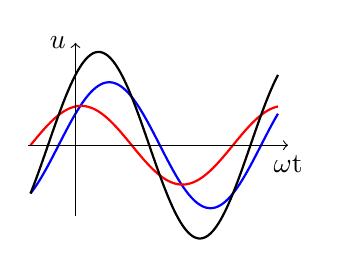
\begin{tikzpicture}
	[SinusPlot/.style={domain=-80:360, samples=100, variable=\t, thick},			%Options for sinus plot
	 AxisArrow/.style={->}
	]
	
	\def\LenSca{140};		%The length of the t-Axis will be: (max_domain - min_domain) / LenSca; in [cm]
	\def\Ueins{0.8cm};		%Amplitude der Spannung U1
	\def\Uzwei{0.5cm};		%Amplitude der Spannung U2
	\def\PhiE{30};			%Phasenverschiebung von U1
	\def\PhiZ{80};			%Phasenverschiebung von U2
	
	\draw[SinusPlot, color=blue] plot (\t/\LenSca,{\Ueins*sin(\t+\PhiE)});	%Plot u1 = sin(wt+phi1)
	\draw[SinusPlot, color=red] plot (\t/\LenSca,{\Uzwei*sin(\t+\PhiZ)});	%PLot u2 = sin(wt+phi2)
	\draw[SinusPlot] plot (\t/\LenSca,{\Ueins*sin(\t+\PhiE)+\Uzwei*sin(\t+\PhiZ)});	%Plot addition u1+u2

	\draw[AxisArrow] (0cm,-0.9cm) -- (0cm,\Ueins+\Uzwei) node[at end, left]{$u$};	%Plot y-axis
	\draw[AxisArrow] (-0.6cm,0) -- (2.7,0cm) node[at end, below]{$\omega$t};		%Plot x-axis
	
	

	
	\end{tikzpicture}
	
\end{flushright}	
\end{frame}

%%%%%%%%%%%%%%%%%%%%%%%%%%%%%%%%%%%%%%%%%%%%%%%%%%%%%%%%%%%%%%%%%%%%%%%%%%%%%

\end{document}

